\documentclass[11pt,letterpaper]{article}

% Packages
\usepackage[margin=0.85in]{geometry}
\usepackage{fontspec}
\usepackage{xcolor}
\usepackage{tikz}
\usetikzlibrary{patterns}
\usepackage{tcolorbox}
\usepackage{enumitem}
\usepackage{graphicx}
\usepackage{setspace}
\usepackage{parskip}
\usepackage{multicol}
\usepackage[hidelinks]{hyperref}

% Font setup
\setmainfont{ElMessiri-Regular}[
    Path = ../,
    Extension = .ttf,
    BoldFont = ElMessiri-Regular,
    BoldFeatures = {FakeBold=1.5},
    Scale=1.0
]

% Define colors
\definecolor{purple}{RGB}{138,43,226}
\definecolor{blue}{RGB}{30,144,255}
\definecolor{green}{RGB}{34,139,34}
\definecolor{red}{RGB}{220,20,60}
\definecolor{orange}{RGB}{255,140,0}
\definecolor{lightgray}{RGB}{245,245,245}
\definecolor{darkgray}{RGB}{100,100,100}

% Custom commands for colored text
\newcommand{\purple}[1]{\textcolor{purple}{\textbf{#1}}}
\newcommand{\bluepurple}[1]{\textcolor{blue}{\textbf{#1}}}
\newcommand{\greentext}[1]{\textcolor{green}{\textbf{#1}}}
\newcommand{\redtext}[1]{\textcolor{red}{\textbf{#1}}}
\newcommand{\orangetext}[1]{\textcolor{orange}{\textbf{#1}}}

% Header and footer
\usepackage{fancyhdr}
\pagestyle{fancy}
\fancyhf{}
\renewcommand{\headrulewidth}{0pt}
\renewcommand{\footrulewidth}{0pt}
\fancyfoot[C]{\small\thepage}

% Title formatting
\usepackage{titlesec}
\titleformat{\section}
  {\LARGE\bfseries\sffamily\color{darkgray}}
  {}
  {0em}
  {}
  [\vspace{-0.5em}\rule{\textwidth}{0.5pt}]
\titleformat{\subsection}
  {\Large\bfseries\sffamily\color{darkgray}}
  {}
  {0em}
  {}

% Better spacing
\setlength{\parskip}{0.6em}
\setstretch{1.15}

\begin{document}

\thispagestyle{empty}

\vspace*{\fill}

% HEADER
\begin{center}
{\Huge\bfseries\sffamily Come Together}

\vspace{0.3cm}

{\LARGE by The Beatles}

\vspace{0.5cm}


\begin{tikzpicture}
    % Decorative music notes
    \fill[purple] (0,0) circle (0.2cm);
    \draw[purple, line width=1.5pt] (0.2,0) -- (0.2,1);
    \fill[blue] (1,0.2) circle (0.2cm);
    \draw[blue, line width=1.5pt] (1.2,0.2) -- (1.2,1.2);
    \fill[green] (2,0) circle (0.2cm);
    \draw[green, line width=1.5pt] (2.2,0) -- (2.2,1);
\end{tikzpicture}

\vspace{0.5cm}

\rule{0.8\textwidth}{0.5pt}
\end{center}

\vspace{0.5cm}

% SONG DETAILS BOX
\begin{tcolorbox}[colback=lightgray,colframe=purple,width=\textwidth,arc=3mm,boxrule=1pt]
\begin{multicols}{2}
\textbf{\purple{BPM:}} 82

\textbf{\bluepurple{Key:}} D minor

\textbf{\greentext{Year:}} 1969

\textbf{\orangetext{Album:}} Abbey Road

\textbf{\redtext{Genre:}} Rock, Blues Rock, Psychedelic Rock
\end{multicols}
\end{tcolorbox}

\vspace*{\fill}

% NEW PAGE FOR PIANO ROLL
\newpage
\thispagestyle{empty}

% Adjust geometry for piano roll page
\newgeometry{top=0.4in, bottom=0.65in, left=0.75in, right=0.75in}

\begin{center}
{\Huge\bfseries Come Together}
\end{center}

\vspace{0.05cm}

\noindent\hspace{2.5cm}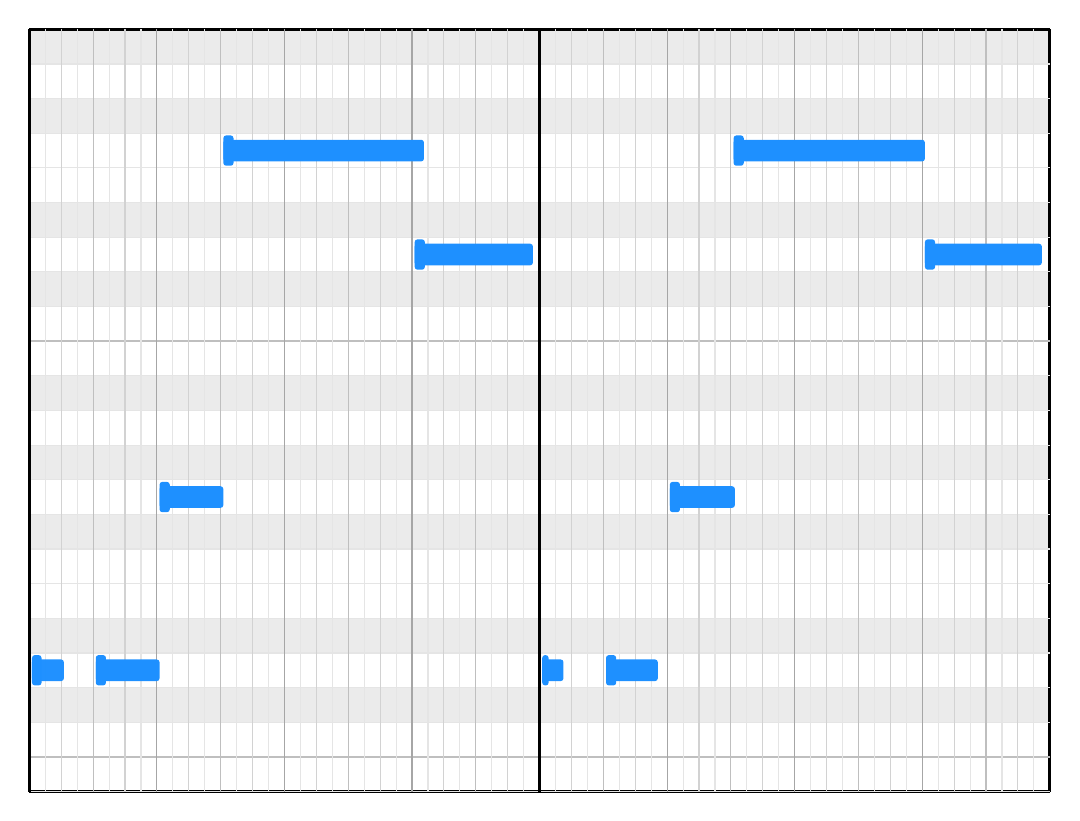
\begin{tikzpicture}[xscale=1.62, yscale=1.1]
\fill[black!8] (0,0.8) rectangle (8,1.2000000000000002);
\fill[black!8] (0,1.6) rectangle (8,2.0);
\fill[black!8] (0,2.8000000000000003) rectangle (8,3.2);
\fill[black!8] (0,3.6) rectangle (8,4.0);
\fill[black!8] (0,4.4) rectangle (8,4.800000000000001);
\fill[black!8] (0,5.6000000000000005) rectangle (8,6.000000000000001);
\fill[black!8] (0,6.4) rectangle (8,6.800000000000001);
\fill[black!8] (0,7.6000000000000005) rectangle (8,8.0);
\fill[black!8] (0,8.4) rectangle (8,8.8);
\draw[black, very thick] (0,0) -- (8,0);
\draw[black, very thick] (0,8.8) -- (8,8.8);
\draw[black, very thick] (8,0) -- (8,8.8);
\draw[gray!20] (0,0.0) -- (8,0.0);
\draw[gray!50, thick] (0,0.4) -- (8,0.4);
\draw[gray!20] (0,0.8) -- (8,0.8);
\draw[gray!20] (0,1.2000000000000002) -- (8,1.2000000000000002);
\draw[gray!20] (0,1.6) -- (8,1.6);
\draw[gray!20] (0,2.0) -- (8,2.0);
\draw[gray!20] (0,2.4000000000000004) -- (8,2.4000000000000004);
\draw[gray!20] (0,2.8000000000000003) -- (8,2.8000000000000003);
\draw[gray!20] (0,3.2) -- (8,3.2);
\draw[gray!20] (0,3.6) -- (8,3.6);
\draw[gray!20] (0,4.0) -- (8,4.0);
\draw[gray!20] (0,4.4) -- (8,4.4);
\draw[gray!20] (0,4.800000000000001) -- (8,4.800000000000001);
\draw[gray!50, thick] (0,5.2) -- (8,5.2);
\draw[gray!20] (0,5.6000000000000005) -- (8,5.6000000000000005);
\draw[gray!20] (0,6.0) -- (8,6.0);
\draw[gray!20] (0,6.4) -- (8,6.4);
\draw[gray!20] (0,6.800000000000001) -- (8,6.800000000000001);
\draw[gray!20] (0,7.2) -- (8,7.2);
\draw[gray!20] (0,7.6000000000000005) -- (8,7.6000000000000005);
\draw[gray!20] (0,8.0) -- (8,8.0);
\draw[gray!20] (0,8.4) -- (8,8.4);
\draw[black, very thick] (0.0,0) -- (0.0,8.8);
\draw[gray!20] (0.125,0) -- (0.125,8.8);
\draw[gray!35] (0.25,0) -- (0.25,8.8);
\draw[gray!20] (0.375,0) -- (0.375,8.8);
\draw[gray!50] (0.5,0) -- (0.5,8.8);
\draw[gray!20] (0.625,0) -- (0.625,8.8);
\draw[gray!35] (0.75,0) -- (0.75,8.8);
\draw[gray!20] (0.875,0) -- (0.875,8.8);
\draw[gray!70] (1.0,0) -- (1.0,8.8);
\draw[gray!20] (1.125,0) -- (1.125,8.8);
\draw[gray!35] (1.25,0) -- (1.25,8.8);
\draw[gray!20] (1.375,0) -- (1.375,8.8);
\draw[gray!50] (1.5,0) -- (1.5,8.8);
\draw[gray!20] (1.625,0) -- (1.625,8.8);
\draw[gray!35] (1.75,0) -- (1.75,8.8);
\draw[gray!20] (1.875,0) -- (1.875,8.8);
\draw[gray!70] (2.0,0) -- (2.0,8.8);
\draw[gray!20] (2.125,0) -- (2.125,8.8);
\draw[gray!35] (2.25,0) -- (2.25,8.8);
\draw[gray!20] (2.375,0) -- (2.375,8.8);
\draw[gray!50] (2.5,0) -- (2.5,8.8);
\draw[gray!20] (2.625,0) -- (2.625,8.8);
\draw[gray!35] (2.75,0) -- (2.75,8.8);
\draw[gray!20] (2.875,0) -- (2.875,8.8);
\draw[gray!70] (3.0,0) -- (3.0,8.8);
\draw[gray!20] (3.125,0) -- (3.125,8.8);
\draw[gray!35] (3.25,0) -- (3.25,8.8);
\draw[gray!20] (3.375,0) -- (3.375,8.8);
\draw[gray!50] (3.5,0) -- (3.5,8.8);
\draw[gray!20] (3.625,0) -- (3.625,8.8);
\draw[gray!35] (3.75,0) -- (3.75,8.8);
\draw[gray!20] (3.875,0) -- (3.875,8.8);
\draw[black, very thick] (4.0,0) -- (4.0,8.8);
\draw[gray!20] (4.125,0) -- (4.125,8.8);
\draw[gray!35] (4.25,0) -- (4.25,8.8);
\draw[gray!20] (4.375,0) -- (4.375,8.8);
\draw[gray!50] (4.5,0) -- (4.5,8.8);
\draw[gray!20] (4.625,0) -- (4.625,8.8);
\draw[gray!35] (4.75,0) -- (4.75,8.8);
\draw[gray!20] (4.875,0) -- (4.875,8.8);
\draw[gray!70] (5.0,0) -- (5.0,8.8);
\draw[gray!20] (5.125,0) -- (5.125,8.8);
\draw[gray!35] (5.25,0) -- (5.25,8.8);
\draw[gray!20] (5.375,0) -- (5.375,8.8);
\draw[gray!50] (5.5,0) -- (5.5,8.8);
\draw[gray!20] (5.625,0) -- (5.625,8.8);
\draw[gray!35] (5.75,0) -- (5.75,8.8);
\draw[gray!20] (5.875,0) -- (5.875,8.8);
\draw[gray!70] (6.0,0) -- (6.0,8.8);
\draw[gray!20] (6.125,0) -- (6.125,8.8);
\draw[gray!35] (6.25,0) -- (6.25,8.8);
\draw[gray!20] (6.375,0) -- (6.375,8.8);
\draw[gray!50] (6.5,0) -- (6.5,8.8);
\draw[gray!20] (6.625,0) -- (6.625,8.8);
\draw[gray!35] (6.75,0) -- (6.75,8.8);
\draw[gray!20] (6.875,0) -- (6.875,8.8);
\draw[gray!70] (7.0,0) -- (7.0,8.8);
\draw[gray!20] (7.125,0) -- (7.125,8.8);
\draw[gray!35] (7.25,0) -- (7.25,8.8);
\draw[gray!20] (7.375,0) -- (7.375,8.8);
\draw[gray!50] (7.5,0) -- (7.5,8.8);
\draw[gray!20] (7.625,0) -- (7.625,8.8);
\draw[gray!35] (7.75,0) -- (7.75,8.8);
\draw[gray!20] (7.875,0) -- (7.875,8.8);
\node[anchor=east, font=\small, overlay] at (-0.3,0.2) {B0};
\node[anchor=east, font=\small\bfseries, overlay] at (-0.3,0.6000000000000001) {C1};
\node[anchor=east, font=\small, overlay] at (-0.3,1.0) {C\#1};
\node[anchor=east, font=\small, overlay] at (-0.3,1.4000000000000001) {D1};
\node[anchor=east, font=\small, overlay] at (-0.3,1.8) {D\#1};
\node[anchor=east, font=\small, overlay] at (-0.3,2.2) {E1};
\node[anchor=east, font=\small, overlay] at (-0.3,2.6000000000000005) {F1};
\node[anchor=east, font=\small, overlay] at (-0.3,3.0000000000000004) {F\#1};
\node[anchor=east, font=\small, overlay] at (-0.3,3.4000000000000004) {G1};
\node[anchor=east, font=\small, overlay] at (-0.3,3.8000000000000003) {G\#1};
\node[anchor=east, font=\small, overlay] at (-0.3,4.2) {A1};
\node[anchor=east, font=\small, overlay] at (-0.3,4.6000000000000005) {A\#1};
\node[anchor=east, font=\small, overlay] at (-0.3,5.000000000000001) {B1};
\node[anchor=east, font=\small\bfseries, overlay] at (-0.3,5.4) {C2};
\node[anchor=east, font=\small, overlay] at (-0.3,5.800000000000001) {C\#2};
\node[anchor=east, font=\small, overlay] at (-0.3,6.2) {D2};
\node[anchor=east, font=\small, overlay] at (-0.3,6.6000000000000005) {D\#2};
\node[anchor=east, font=\small, overlay] at (-0.3,7.000000000000001) {E2};
\node[anchor=east, font=\small, overlay] at (-0.3,7.4) {F2};
\node[anchor=east, font=\small, overlay] at (-0.3,7.800000000000001) {F\#2};
\node[anchor=east, font=\small, overlay] at (-0.3,8.2) {G2};
\node[anchor=east, font=\small, overlay] at (-0.3,8.6) {G\#2};
\fill[blue, opacity=0.99, rounded corners=1pt] (0.020833333333333332,1.2750000000000001) rectangle (0.2708333333333333,1.5250000000000001);
\fill[blue, opacity=1.0, rounded corners=1pt] (0.020833333333333332,1.225) rectangle (0.09583333333333333,1.5750000000000002);
\fill[blue, opacity=1.00, rounded corners=1pt] (0.5208333333333334,1.2750000000000001) rectangle (1.0208333333333335,1.5250000000000001);
\fill[blue, opacity=1.0, rounded corners=1pt] (0.5208333333333334,1.225) rectangle (0.6008333333333333,1.5750000000000002);
\fill[blue, opacity=1.00, rounded corners=1pt] (1.0208333333333333,3.275) rectangle (1.5208333333333333,3.525);
\fill[blue, opacity=1.0, rounded corners=1pt] (1.0208333333333333,3.225) rectangle (1.1008333333333333,3.575);
\fill[blue, opacity=1.00, rounded corners=1pt] (1.5208333333333333,7.275) rectangle (3.09375,7.525);
\fill[blue, opacity=1.0, rounded corners=1pt] (1.5208333333333333,7.2250000000000005) rectangle (1.6008333333333333,7.575);
\fill[blue, opacity=1.00, rounded corners=1pt] (3.0208333333333335,6.075) rectangle (3.947916666666667,6.325);
\fill[blue, opacity=1.0, rounded corners=1pt] (3.0208333333333335,6.025) rectangle (3.1008333333333336,6.375);
\fill[blue, opacity=1.00, rounded corners=1pt] (4.020833333333333,1.2750000000000001) rectangle (4.1875,1.5250000000000001);
\fill[blue, opacity=1.0, rounded corners=1pt] (4.020833333333333,1.225) rectangle (4.070833333333333,1.5750000000000002);
\fill[blue, opacity=1.00, rounded corners=1pt] (4.520833333333333,1.2750000000000001) rectangle (4.927083333333333,1.5250000000000001);
\fill[blue, opacity=1.0, rounded corners=1pt] (4.520833333333333,1.225) rectangle (4.600833333333333,1.5750000000000002);
\fill[blue, opacity=1.00, rounded corners=1pt] (5.020833333333333,3.275) rectangle (5.53125,3.525);
\fill[blue, opacity=1.0, rounded corners=1pt] (5.020833333333333,3.225) rectangle (5.100833333333333,3.575);
\fill[blue, opacity=1.00, rounded corners=1pt] (5.520833333333333,7.275) rectangle (7.020833333333333,7.525);
\fill[blue, opacity=1.0, rounded corners=1pt] (5.520833333333333,7.2250000000000005) rectangle (5.600833333333333,7.575);
\fill[blue, opacity=1.00, rounded corners=1pt] (7.020833333333333,6.075) rectangle (7.9375,6.325);
\fill[blue, opacity=1.0, rounded corners=1pt] (7.020833333333333,6.025) rectangle (7.100833333333333,6.375);
\node[rotate=90, font=\Large\bfseries, overlay] at (8.5,4.4) {BASS};
\end{tikzpicture}

\vspace{0.05cm}

\noindent\hspace{2.5cm}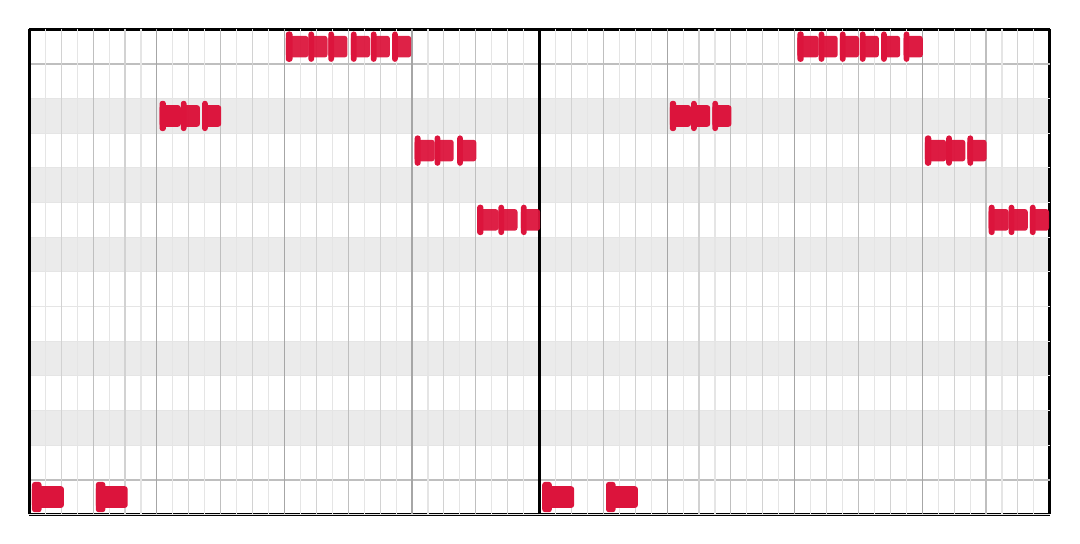
\begin{tikzpicture}[xscale=1.62, yscale=1.1]
\fill[black!8] (0,0.8) rectangle (8,1.2000000000000002);
\fill[black!8] (0,1.6) rectangle (8,2.0);
\fill[black!8] (0,2.8000000000000003) rectangle (8,3.2);
\fill[black!8] (0,3.6) rectangle (8,4.0);
\fill[black!8] (0,4.4) rectangle (8,4.800000000000001);
\draw[black, very thick] (0,0) -- (8,0);
\draw[black, very thick] (0,5.6000000000000005) -- (8,5.6000000000000005);
\draw[black, very thick] (8,0) -- (8,5.6000000000000005);
\draw[gray!20] (0,0.0) -- (8,0.0);
\draw[gray!50, thick] (0,0.4) -- (8,0.4);
\draw[gray!20] (0,0.8) -- (8,0.8);
\draw[gray!20] (0,1.2000000000000002) -- (8,1.2000000000000002);
\draw[gray!20] (0,1.6) -- (8,1.6);
\draw[gray!20] (0,2.0) -- (8,2.0);
\draw[gray!20] (0,2.4000000000000004) -- (8,2.4000000000000004);
\draw[gray!20] (0,2.8000000000000003) -- (8,2.8000000000000003);
\draw[gray!20] (0,3.2) -- (8,3.2);
\draw[gray!20] (0,3.6) -- (8,3.6);
\draw[gray!20] (0,4.0) -- (8,4.0);
\draw[gray!20] (0,4.4) -- (8,4.4);
\draw[gray!20] (0,4.800000000000001) -- (8,4.800000000000001);
\draw[gray!50, thick] (0,5.2) -- (8,5.2);
\draw[black, very thick] (0.0,0) -- (0.0,5.6000000000000005);
\draw[gray!20] (0.125,0) -- (0.125,5.6000000000000005);
\draw[gray!35] (0.25,0) -- (0.25,5.6000000000000005);
\draw[gray!20] (0.375,0) -- (0.375,5.6000000000000005);
\draw[gray!50] (0.5,0) -- (0.5,5.6000000000000005);
\draw[gray!20] (0.625,0) -- (0.625,5.6000000000000005);
\draw[gray!35] (0.75,0) -- (0.75,5.6000000000000005);
\draw[gray!20] (0.875,0) -- (0.875,5.6000000000000005);
\draw[gray!70] (1.0,0) -- (1.0,5.6000000000000005);
\draw[gray!20] (1.125,0) -- (1.125,5.6000000000000005);
\draw[gray!35] (1.25,0) -- (1.25,5.6000000000000005);
\draw[gray!20] (1.375,0) -- (1.375,5.6000000000000005);
\draw[gray!50] (1.5,0) -- (1.5,5.6000000000000005);
\draw[gray!20] (1.625,0) -- (1.625,5.6000000000000005);
\draw[gray!35] (1.75,0) -- (1.75,5.6000000000000005);
\draw[gray!20] (1.875,0) -- (1.875,5.6000000000000005);
\draw[gray!70] (2.0,0) -- (2.0,5.6000000000000005);
\draw[gray!20] (2.125,0) -- (2.125,5.6000000000000005);
\draw[gray!35] (2.25,0) -- (2.25,5.6000000000000005);
\draw[gray!20] (2.375,0) -- (2.375,5.6000000000000005);
\draw[gray!50] (2.5,0) -- (2.5,5.6000000000000005);
\draw[gray!20] (2.625,0) -- (2.625,5.6000000000000005);
\draw[gray!35] (2.75,0) -- (2.75,5.6000000000000005);
\draw[gray!20] (2.875,0) -- (2.875,5.6000000000000005);
\draw[gray!70] (3.0,0) -- (3.0,5.6000000000000005);
\draw[gray!20] (3.125,0) -- (3.125,5.6000000000000005);
\draw[gray!35] (3.25,0) -- (3.25,5.6000000000000005);
\draw[gray!20] (3.375,0) -- (3.375,5.6000000000000005);
\draw[gray!50] (3.5,0) -- (3.5,5.6000000000000005);
\draw[gray!20] (3.625,0) -- (3.625,5.6000000000000005);
\draw[gray!35] (3.75,0) -- (3.75,5.6000000000000005);
\draw[gray!20] (3.875,0) -- (3.875,5.6000000000000005);
\draw[black, very thick] (4.0,0) -- (4.0,5.6000000000000005);
\draw[gray!20] (4.125,0) -- (4.125,5.6000000000000005);
\draw[gray!35] (4.25,0) -- (4.25,5.6000000000000005);
\draw[gray!20] (4.375,0) -- (4.375,5.6000000000000005);
\draw[gray!50] (4.5,0) -- (4.5,5.6000000000000005);
\draw[gray!20] (4.625,0) -- (4.625,5.6000000000000005);
\draw[gray!35] (4.75,0) -- (4.75,5.6000000000000005);
\draw[gray!20] (4.875,0) -- (4.875,5.6000000000000005);
\draw[gray!70] (5.0,0) -- (5.0,5.6000000000000005);
\draw[gray!20] (5.125,0) -- (5.125,5.6000000000000005);
\draw[gray!35] (5.25,0) -- (5.25,5.6000000000000005);
\draw[gray!20] (5.375,0) -- (5.375,5.6000000000000005);
\draw[gray!50] (5.5,0) -- (5.5,5.6000000000000005);
\draw[gray!20] (5.625,0) -- (5.625,5.6000000000000005);
\draw[gray!35] (5.75,0) -- (5.75,5.6000000000000005);
\draw[gray!20] (5.875,0) -- (5.875,5.6000000000000005);
\draw[gray!70] (6.0,0) -- (6.0,5.6000000000000005);
\draw[gray!20] (6.125,0) -- (6.125,5.6000000000000005);
\draw[gray!35] (6.25,0) -- (6.25,5.6000000000000005);
\draw[gray!20] (6.375,0) -- (6.375,5.6000000000000005);
\draw[gray!50] (6.5,0) -- (6.5,5.6000000000000005);
\draw[gray!20] (6.625,0) -- (6.625,5.6000000000000005);
\draw[gray!35] (6.75,0) -- (6.75,5.6000000000000005);
\draw[gray!20] (6.875,0) -- (6.875,5.6000000000000005);
\draw[gray!70] (7.0,0) -- (7.0,5.6000000000000005);
\draw[gray!20] (7.125,0) -- (7.125,5.6000000000000005);
\draw[gray!35] (7.25,0) -- (7.25,5.6000000000000005);
\draw[gray!20] (7.375,0) -- (7.375,5.6000000000000005);
\draw[gray!50] (7.5,0) -- (7.5,5.6000000000000005);
\draw[gray!20] (7.625,0) -- (7.625,5.6000000000000005);
\draw[gray!35] (7.75,0) -- (7.75,5.6000000000000005);
\draw[gray!20] (7.875,0) -- (7.875,5.6000000000000005);
\node[anchor=east, font=\small, overlay] at (-0.3,0.2) {Kick};
\node[anchor=east, font=\small, overlay] at (-0.3,0.6000000000000001) {Kick};
\node[anchor=east, font=\small, overlay] at (-0.3,1.0) {Side Stick};
\node[anchor=east, font=\small, overlay] at (-0.3,1.4000000000000001) {Snare};
\node[anchor=east, font=\small, overlay] at (-0.3,1.8) {Clap};
\node[anchor=east, font=\small, overlay] at (-0.3,2.2) {Snare};
\node[anchor=east, font=\small, overlay] at (-0.3,2.6000000000000005) {Tom Low};
\node[anchor=east, font=\small, overlay] at (-0.3,3.0000000000000004) {Hi-Hat Closed};
\node[anchor=east, font=\small, overlay] at (-0.3,3.4000000000000004) {Tom Low-Mid};
\node[anchor=east, font=\small, overlay] at (-0.3,3.8000000000000003) {Hi-Hat Pedal};
\node[anchor=east, font=\small, overlay] at (-0.3,4.2) {Tom Mid};
\node[anchor=east, font=\small, overlay] at (-0.3,4.6000000000000005) {Hi-Hat Open};
\node[anchor=east, font=\small, overlay] at (-0.3,5.000000000000001) {Tom Mid-High};
\node[anchor=east, font=\small, overlay] at (-0.3,5.4) {Tom High};
\fill[red, opacity=1.00, rounded corners=1pt] (0.020833333333333332,0.07499999999999998) rectangle (0.2708333333333333,0.32499999999999996);
\fill[red, opacity=1.0, rounded corners=1pt] (0.020833333333333332,0.025) rectangle (0.09583333333333333,0.375);
\fill[red, opacity=1.00, rounded corners=1pt] (0.5208333333333334,0.07499999999999998) rectangle (0.7708333333333334,0.32499999999999996);
\fill[red, opacity=1.0, rounded corners=1pt] (0.5208333333333334,0.025) rectangle (0.5958333333333333,0.375);
\fill[red, opacity=1.00, rounded corners=1pt] (1.0208333333333333,4.4750000000000005) rectangle (1.1875,4.7250000000000005);
\fill[red, opacity=1.0, rounded corners=1pt] (1.0208333333333333,4.425000000000001) rectangle (1.0708333333333333,4.775);
\fill[red, opacity=0.98, rounded corners=1pt] (1.1875,4.4750000000000005) rectangle (1.3375,4.7250000000000005);
\fill[red, opacity=1.0, rounded corners=1pt] (1.1875,4.425000000000001) rectangle (1.2325,4.775);
\fill[red, opacity=0.99, rounded corners=1pt] (1.3541666666666667,4.4750000000000005) rectangle (1.5041666666666667,4.7250000000000005);
\fill[red, opacity=1.0, rounded corners=1pt] (1.3541666666666667,4.425000000000001) rectangle (1.3991666666666667,4.775);
\fill[red, opacity=0.94, rounded corners=1pt] (2.0104166666666665,5.275) rectangle (2.1875,5.525);
\fill[red, opacity=1.0, rounded corners=1pt] (2.0104166666666665,5.2250000000000005) rectangle (2.0635416666666666,5.575);
\fill[red, opacity=0.94, rounded corners=1pt] (2.1875,5.275) rectangle (2.3375,5.525);
\fill[red, opacity=1.0, rounded corners=1pt] (2.1875,5.2250000000000005) rectangle (2.2325,5.575);
\fill[red, opacity=0.94, rounded corners=1pt] (2.34375,5.275) rectangle (2.49375,5.525);
\fill[red, opacity=1.0, rounded corners=1pt] (2.34375,5.2250000000000005) rectangle (2.38875,5.575);
\fill[red, opacity=0.94, rounded corners=1pt] (2.5208333333333335,5.275) rectangle (2.6708333333333334,5.525);
\fill[red, opacity=1.0, rounded corners=1pt] (2.5208333333333335,5.2250000000000005) rectangle (2.5658333333333334,5.575);
\fill[red, opacity=0.94, rounded corners=1pt] (2.6770833333333335,5.275) rectangle (2.8270833333333334,5.525);
\fill[red, opacity=1.0, rounded corners=1pt] (2.6770833333333335,5.2250000000000005) rectangle (2.7220833333333334,5.575);
\fill[red, opacity=0.94, rounded corners=1pt] (2.84375,5.275) rectangle (2.99375,5.525);
\fill[red, opacity=1.0, rounded corners=1pt] (2.84375,5.2250000000000005) rectangle (2.88875,5.575);
\fill[red, opacity=0.95, rounded corners=1pt] (3.0208333333333335,4.075) rectangle (3.1770833333333335,4.325);
\fill[red, opacity=1.0, rounded corners=1pt] (3.0208333333333335,4.025) rectangle (3.0677083333333335,4.375);
\fill[red, opacity=0.95, rounded corners=1pt] (3.1770833333333335,4.075) rectangle (3.3270833333333334,4.325);
\fill[red, opacity=1.0, rounded corners=1pt] (3.1770833333333335,4.025) rectangle (3.2220833333333334,4.375);
\fill[red, opacity=0.95, rounded corners=1pt] (3.3541666666666665,4.075) rectangle (3.5041666666666664,4.325);
\fill[red, opacity=1.0, rounded corners=1pt] (3.3541666666666665,4.025) rectangle (3.3991666666666664,4.375);
\fill[red, opacity=0.95, rounded corners=1pt] (3.5104166666666665,3.275) rectangle (3.677083333333333,3.525);
\fill[red, opacity=1.0, rounded corners=1pt] (3.5104166666666665,3.225) rectangle (3.5604166666666663,3.575);
\fill[red, opacity=0.95, rounded corners=1pt] (3.6770833333333335,3.275) rectangle (3.8270833333333334,3.525);
\fill[red, opacity=1.0, rounded corners=1pt] (3.6770833333333335,3.225) rectangle (3.7220833333333334,3.575);
\fill[red, opacity=0.95, rounded corners=1pt] (3.8541666666666665,3.275) rectangle (4.004166666666666,3.525);
\fill[red, opacity=1.0, rounded corners=1pt] (3.8541666666666665,3.225) rectangle (3.8991666666666664,3.575);
\fill[red, opacity=1.00, rounded corners=1pt] (4.020833333333333,0.07499999999999998) rectangle (4.270833333333333,0.32499999999999996);
\fill[red, opacity=1.0, rounded corners=1pt] (4.020833333333333,0.025) rectangle (4.095833333333333,0.375);
\fill[red, opacity=1.00, rounded corners=1pt] (4.520833333333333,0.07499999999999998) rectangle (4.770833333333333,0.32499999999999996);
\fill[red, opacity=1.0, rounded corners=1pt] (4.520833333333333,0.025) rectangle (4.595833333333333,0.375);
\fill[red, opacity=1.00, rounded corners=1pt] (5.020833333333333,4.4750000000000005) rectangle (5.1875,4.7250000000000005);
\fill[red, opacity=1.0, rounded corners=1pt] (5.020833333333333,4.425000000000001) rectangle (5.070833333333333,4.775);
\fill[red, opacity=1.00, rounded corners=1pt] (5.1875,4.4750000000000005) rectangle (5.3375,4.7250000000000005);
\fill[red, opacity=1.0, rounded corners=1pt] (5.1875,4.425000000000001) rectangle (5.2325,4.775);
\fill[red, opacity=0.99, rounded corners=1pt] (5.354166666666667,4.4750000000000005) rectangle (5.504166666666667,4.7250000000000005);
\fill[red, opacity=1.0, rounded corners=1pt] (5.354166666666667,4.425000000000001) rectangle (5.399166666666667,4.775);
\fill[red, opacity=0.97, rounded corners=1pt] (6.020833333333333,5.275) rectangle (6.1875,5.525);
\fill[red, opacity=1.0, rounded corners=1pt] (6.020833333333333,5.2250000000000005) rectangle (6.070833333333333,5.575);
\fill[red, opacity=0.97, rounded corners=1pt] (6.1875,5.275) rectangle (6.3375,5.525);
\fill[red, opacity=1.0, rounded corners=1pt] (6.1875,5.2250000000000005) rectangle (6.2325,5.575);
\fill[red, opacity=0.97, rounded corners=1pt] (6.354166666666667,5.275) rectangle (6.504166666666667,5.525);
\fill[red, opacity=1.0, rounded corners=1pt] (6.354166666666667,5.2250000000000005) rectangle (6.399166666666667,5.575);
\fill[red, opacity=0.97, rounded corners=1pt] (6.510416666666667,5.275) rectangle (6.660416666666667,5.525);
\fill[red, opacity=1.0, rounded corners=1pt] (6.510416666666667,5.2250000000000005) rectangle (6.555416666666667,5.575);
\fill[red, opacity=0.97, rounded corners=1pt] (6.677083333333333,5.275) rectangle (6.827083333333333,5.525);
\fill[red, opacity=1.0, rounded corners=1pt] (6.677083333333333,5.2250000000000005) rectangle (6.722083333333333,5.575);
\fill[red, opacity=0.97, rounded corners=1pt] (6.854166666666667,5.275) rectangle (7.004166666666667,5.525);
\fill[red, opacity=1.0, rounded corners=1pt] (6.854166666666667,5.2250000000000005) rectangle (6.899166666666667,5.575);
\fill[red, opacity=0.97, rounded corners=1pt] (7.020833333333333,4.075) rectangle (7.1875,4.325);
\fill[red, opacity=1.0, rounded corners=1pt] (7.020833333333333,4.025) rectangle (7.070833333333333,4.375);
\fill[red, opacity=0.97, rounded corners=1pt] (7.1875,4.075) rectangle (7.3375,4.325);
\fill[red, opacity=1.0, rounded corners=1pt] (7.1875,4.025) rectangle (7.2325,4.375);
\fill[red, opacity=0.97, rounded corners=1pt] (7.354166666666667,4.075) rectangle (7.504166666666667,4.325);
\fill[red, opacity=1.0, rounded corners=1pt] (7.354166666666667,4.025) rectangle (7.399166666666667,4.375);
\fill[red, opacity=0.97, rounded corners=1pt] (7.520833333333333,3.275) rectangle (7.677083333333333,3.525);
\fill[red, opacity=1.0, rounded corners=1pt] (7.520833333333333,3.225) rectangle (7.567708333333333,3.575);
\fill[red, opacity=0.97, rounded corners=1pt] (7.677083333333333,3.275) rectangle (7.827083333333333,3.525);
\fill[red, opacity=1.0, rounded corners=1pt] (7.677083333333333,3.225) rectangle (7.722083333333333,3.575);
\fill[red, opacity=0.97, rounded corners=1pt] (7.84375,3.275) rectangle (7.99375,3.525);
\fill[red, opacity=1.0, rounded corners=1pt] (7.84375,3.225) rectangle (7.88875,3.575);
\node[rotate=90, font=\Large\bfseries, overlay] at (8.5,2.8000000000000003) {DRUMS};
\end{tikzpicture}

\vspace{0.05cm}

\noindent\hspace{2.5cm}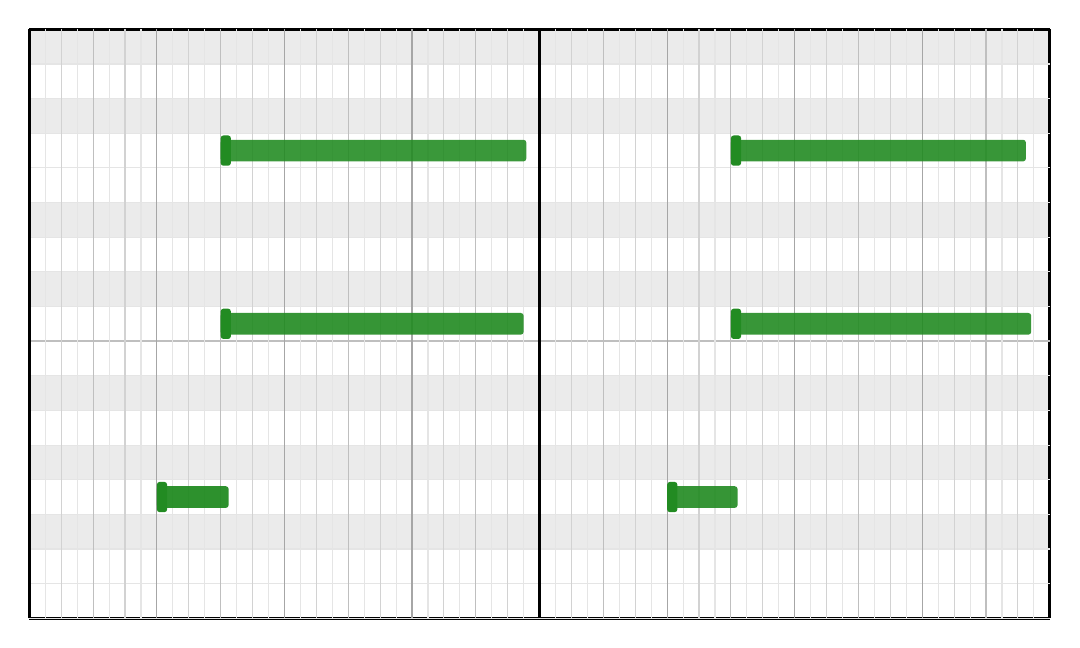
\begin{tikzpicture}[xscale=1.62, yscale=1.1]
\fill[black!8] (0,0.8) rectangle (8,1.2000000000000002);
\fill[black!8] (0,1.6) rectangle (8,2.0);
\fill[black!8] (0,2.4000000000000004) rectangle (8,2.8000000000000003);
\fill[black!8] (0,3.6) rectangle (8,4.0);
\fill[black!8] (0,4.4) rectangle (8,4.800000000000001);
\fill[black!8] (0,5.6000000000000005) rectangle (8,6.000000000000001);
\fill[black!8] (0,6.4) rectangle (8,6.800000000000001);
\draw[black, very thick] (0,0) -- (8,0);
\draw[black, very thick] (0,6.800000000000001) -- (8,6.800000000000001);
\draw[black, very thick] (8,0) -- (8,6.800000000000001);
\draw[gray!20] (0,0.0) -- (8,0.0);
\draw[gray!20] (0,0.4) -- (8,0.4);
\draw[gray!20] (0,0.8) -- (8,0.8);
\draw[gray!20] (0,1.2000000000000002) -- (8,1.2000000000000002);
\draw[gray!20] (0,1.6) -- (8,1.6);
\draw[gray!20] (0,2.0) -- (8,2.0);
\draw[gray!20] (0,2.4000000000000004) -- (8,2.4000000000000004);
\draw[gray!20] (0,2.8000000000000003) -- (8,2.8000000000000003);
\draw[gray!50, thick] (0,3.2) -- (8,3.2);
\draw[gray!20] (0,3.6) -- (8,3.6);
\draw[gray!20] (0,4.0) -- (8,4.0);
\draw[gray!20] (0,4.4) -- (8,4.4);
\draw[gray!20] (0,4.800000000000001) -- (8,4.800000000000001);
\draw[gray!20] (0,5.2) -- (8,5.2);
\draw[gray!20] (0,5.6000000000000005) -- (8,5.6000000000000005);
\draw[gray!20] (0,6.0) -- (8,6.0);
\draw[gray!20] (0,6.4) -- (8,6.4);
\draw[black, very thick] (0.0,0) -- (0.0,6.800000000000001);
\node[below, font=\large\bfseries, overlay] at (0.0,-0.5) {Bar 1};
\draw[gray!20] (0.125,0) -- (0.125,6.800000000000001);
\draw[gray!35] (0.25,0) -- (0.25,6.800000000000001);
\draw[gray!20] (0.375,0) -- (0.375,6.800000000000001);
\draw[gray!50] (0.5,0) -- (0.5,6.800000000000001);
\draw[gray!20] (0.625,0) -- (0.625,6.800000000000001);
\draw[gray!35] (0.75,0) -- (0.75,6.800000000000001);
\draw[gray!20] (0.875,0) -- (0.875,6.800000000000001);
\draw[gray!70] (1.0,0) -- (1.0,6.800000000000001);
\node[below, font=\small, gray, overlay] at (1.0,-0.5) {2};
\draw[gray!20] (1.125,0) -- (1.125,6.800000000000001);
\draw[gray!35] (1.25,0) -- (1.25,6.800000000000001);
\draw[gray!20] (1.375,0) -- (1.375,6.800000000000001);
\draw[gray!50] (1.5,0) -- (1.5,6.800000000000001);
\draw[gray!20] (1.625,0) -- (1.625,6.800000000000001);
\draw[gray!35] (1.75,0) -- (1.75,6.800000000000001);
\draw[gray!20] (1.875,0) -- (1.875,6.800000000000001);
\draw[gray!70] (2.0,0) -- (2.0,6.800000000000001);
\node[below, font=\small, gray, overlay] at (2.0,-0.5) {3};
\draw[gray!20] (2.125,0) -- (2.125,6.800000000000001);
\draw[gray!35] (2.25,0) -- (2.25,6.800000000000001);
\draw[gray!20] (2.375,0) -- (2.375,6.800000000000001);
\draw[gray!50] (2.5,0) -- (2.5,6.800000000000001);
\draw[gray!20] (2.625,0) -- (2.625,6.800000000000001);
\draw[gray!35] (2.75,0) -- (2.75,6.800000000000001);
\draw[gray!20] (2.875,0) -- (2.875,6.800000000000001);
\draw[gray!70] (3.0,0) -- (3.0,6.800000000000001);
\node[below, font=\small, gray, overlay] at (3.0,-0.5) {4};
\draw[gray!20] (3.125,0) -- (3.125,6.800000000000001);
\draw[gray!35] (3.25,0) -- (3.25,6.800000000000001);
\draw[gray!20] (3.375,0) -- (3.375,6.800000000000001);
\draw[gray!50] (3.5,0) -- (3.5,6.800000000000001);
\draw[gray!20] (3.625,0) -- (3.625,6.800000000000001);
\draw[gray!35] (3.75,0) -- (3.75,6.800000000000001);
\draw[gray!20] (3.875,0) -- (3.875,6.800000000000001);
\draw[black, very thick] (4.0,0) -- (4.0,6.800000000000001);
\node[below, font=\large\bfseries, overlay] at (4.0,-0.5) {Bar 2};
\draw[gray!20] (4.125,0) -- (4.125,6.800000000000001);
\draw[gray!35] (4.25,0) -- (4.25,6.800000000000001);
\draw[gray!20] (4.375,0) -- (4.375,6.800000000000001);
\draw[gray!50] (4.5,0) -- (4.5,6.800000000000001);
\draw[gray!20] (4.625,0) -- (4.625,6.800000000000001);
\draw[gray!35] (4.75,0) -- (4.75,6.800000000000001);
\draw[gray!20] (4.875,0) -- (4.875,6.800000000000001);
\draw[gray!70] (5.0,0) -- (5.0,6.800000000000001);
\node[below, font=\small, gray, overlay] at (5.0,-0.5) {2};
\draw[gray!20] (5.125,0) -- (5.125,6.800000000000001);
\draw[gray!35] (5.25,0) -- (5.25,6.800000000000001);
\draw[gray!20] (5.375,0) -- (5.375,6.800000000000001);
\draw[gray!50] (5.5,0) -- (5.5,6.800000000000001);
\draw[gray!20] (5.625,0) -- (5.625,6.800000000000001);
\draw[gray!35] (5.75,0) -- (5.75,6.800000000000001);
\draw[gray!20] (5.875,0) -- (5.875,6.800000000000001);
\draw[gray!70] (6.0,0) -- (6.0,6.800000000000001);
\node[below, font=\small, gray, overlay] at (6.0,-0.5) {3};
\draw[gray!20] (6.125,0) -- (6.125,6.800000000000001);
\draw[gray!35] (6.25,0) -- (6.25,6.800000000000001);
\draw[gray!20] (6.375,0) -- (6.375,6.800000000000001);
\draw[gray!50] (6.5,0) -- (6.5,6.800000000000001);
\draw[gray!20] (6.625,0) -- (6.625,6.800000000000001);
\draw[gray!35] (6.75,0) -- (6.75,6.800000000000001);
\draw[gray!20] (6.875,0) -- (6.875,6.800000000000001);
\draw[gray!70] (7.0,0) -- (7.0,6.800000000000001);
\node[below, font=\small, gray, overlay] at (7.0,-0.5) {4};
\draw[gray!20] (7.125,0) -- (7.125,6.800000000000001);
\draw[gray!35] (7.25,0) -- (7.25,6.800000000000001);
\draw[gray!20] (7.375,0) -- (7.375,6.800000000000001);
\draw[gray!50] (7.5,0) -- (7.5,6.800000000000001);
\draw[gray!20] (7.625,0) -- (7.625,6.800000000000001);
\draw[gray!35] (7.75,0) -- (7.75,6.800000000000001);
\draw[gray!20] (7.875,0) -- (7.875,6.800000000000001);
\node[anchor=east, font=\small, overlay] at (-0.3,0.2) {E3};
\node[anchor=east, font=\small, overlay] at (-0.3,0.6000000000000001) {F3};
\node[anchor=east, font=\small, overlay] at (-0.3,1.0) {F\#3};
\node[anchor=east, font=\small, overlay] at (-0.3,1.4000000000000001) {G3};
\node[anchor=east, font=\small, overlay] at (-0.3,1.8) {G\#3};
\node[anchor=east, font=\small, overlay] at (-0.3,2.2) {A3};
\node[anchor=east, font=\small, overlay] at (-0.3,2.6000000000000005) {A\#3};
\node[anchor=east, font=\small, overlay] at (-0.3,3.0000000000000004) {B3};
\node[anchor=east, font=\small\bfseries, overlay] at (-0.3,3.4000000000000004) {C4};
\node[anchor=east, font=\small, overlay] at (-0.3,3.8000000000000003) {C\#4};
\node[anchor=east, font=\small, overlay] at (-0.3,4.2) {D4};
\node[anchor=east, font=\small, overlay] at (-0.3,4.6000000000000005) {D\#4};
\node[anchor=east, font=\small, overlay] at (-0.3,5.000000000000001) {E4};
\node[anchor=east, font=\small, overlay] at (-0.3,5.4) {F4};
\node[anchor=east, font=\small, overlay] at (-0.3,5.800000000000001) {F\#4};
\node[anchor=east, font=\small, overlay] at (-0.3,6.2) {G4};
\node[anchor=east, font=\small, overlay] at (-0.3,6.6000000000000005) {G\#4};
\fill[green, opacity=0.95, rounded corners=1pt] (1.0,1.2750000000000001) rectangle (1.5625,1.5250000000000001);
\fill[green, opacity=1.0, rounded corners=1pt] (1.0,1.225) rectangle (1.08,1.5750000000000002);
\fill[green, opacity=0.91, rounded corners=1pt] (1.5,3.275) rectangle (3.875,3.525);
\fill[green, opacity=1.0, rounded corners=1pt] (1.5,3.225) rectangle (1.58,3.575);
\fill[green, opacity=0.89, rounded corners=1pt] (1.5,5.275) rectangle (3.8958333333333335,5.525);
\fill[green, opacity=1.0, rounded corners=1pt] (1.5,5.2250000000000005) rectangle (1.58,5.575);
\fill[green, opacity=0.91, rounded corners=1pt] (5.0,1.2750000000000001) rectangle (5.552083333333333,1.5250000000000001);
\fill[green, opacity=1.0, rounded corners=1pt] (5.0,1.225) rectangle (5.08,1.5750000000000002);
\fill[green, opacity=0.90, rounded corners=1pt] (5.5,5.275) rectangle (7.8125,5.525);
\fill[green, opacity=1.0, rounded corners=1pt] (5.5,5.2250000000000005) rectangle (5.58,5.575);
\fill[green, opacity=0.90, rounded corners=1pt] (5.5,3.275) rectangle (7.854166666666666,3.525);
\fill[green, opacity=1.0, rounded corners=1pt] (5.5,3.225) rectangle (5.58,3.575);
\node[rotate=90, font=\Large\bfseries, overlay] at (8.5,3.4000000000000004) {KEYS};
\end{tikzpicture}

% Reset geometry for remaining pages
\restoregeometry

% NEW PAGE FOR HISTORY AND CONTENT
\newpage

% ABOUT THE ARTIST
\section*{About The Beatles}

The Beatles were an English rock band formed in Liverpool in 1960. The group consisted of John Lennon, Paul McCartney, George Harrison, and Ringo Starr. They are widely regarded as the most influential band in the history of popular music.

The Beatles revolutionized many aspects of the music industry and were often at the forefront of cultural movements during the 1960s. Their innovative approach to songwriting, recording techniques, and album production set new standards that continue to influence musicians today.

By 1969, when "Come Together" was released, The Beatles were at their creative peak while simultaneously dealing with internal tensions that would eventually lead to their breakup in 1970. Despite these challenges, they continued to produce groundbreaking music that pushed the boundaries of rock and pop.

\vspace{0.5cm}

% ABOUT THE SONG
\section*{About "Come Together"}

"Come Together" is the opening track on The Beatles' iconic 1969 album \textit{Abbey Road}, their penultimate studio album. Written primarily by John Lennon, the song was originally conceived as a campaign song for Timothy Leary's California gubernatorial run against Ronald Reagan in 1969.

The song features one of the most recognizable basslines in rock history, played by Paul McCartney. The groove is built on a swampy, bluesy feel that was somewhat unusual for The Beatles at the time. The cryptic lyrics reference each member of the band in abstract ways, with lines like "He got toe jam football" and "He wear no shoeshine."

\textbf{Cultural Impact:} "Come Together" became a Top 10 hit and has been covered by countless artists across multiple genres. Its infectious groove and mysterious lyrics have made it a staple of classic rock radio and a favorite for musicians to reinterpret.

\textbf{Production Notes:} The track showcases the production genius of The Beatles and George Martin. The distinctive electric piano sound, the tight drums, and the prominent bass create a minimalist but powerful sonic landscape. The "shoot me" backing vocals add to the song's mystique.

\vspace{0.5cm}

% MUSICAL ELEMENTS
\section*{Key Musical Elements}

\subsection*{What Makes This Beat Special:}

\begin{itemize}[leftmargin=*]
\item \textbf{Iconic Bassline:} The sliding, bluesy bass riff is one of the most recognizable in rock history—simple but unforgettable
\item \textbf{The Groove:} Laid-back, swampy feel at 82 BPM creates a hypnotic, almost funky vibe
\item \textbf{Minimal Drums:} Sparse kick and snare pattern lets the bass and vocals breathe
\item \textbf{Electric Piano:} The Fender Rhodes adds texture without cluttering the arrangement
\item \textbf{Space:} What's \textit{not} played is as important as what is—the song uses silence effectively
\end{itemize}

\subsection*{What You'll Learn:}

\begin{itemize}[leftmargin=*]
\item How to create a powerful groove with minimal elements
\item The art of the \purple{bassline}—melodic yet rhythmic
\item Working with \bluepurple{space} in your arrangements
\item Building tension and release through dynamics
\item Creating a hypnotic loop that keeps listeners engaged
\end{itemize}

\vspace{0.5cm}

% COMPARABLE SONGS
\section*{If You Like This, Check Out:}

\begin{tcolorbox}[colback=blue!5,colframe=blue,width=\textwidth,arc=3mm,boxrule=1pt]
\textbf{Similar Grooves \& Vibes:}

\begin{itemize}[leftmargin=*, itemsep=0.3em]
\item \textbf{"Chameleon" - Herbie Hancock} \\
    \textit{Swampy, hypnotic funk bassline with similar laid-back groove}
\item \textbf{"Cissy Strut" - The Meters} \\
    \textit{New Orleans funk with that dirty, swampy bassline feel}
\item \textbf{"Use Me" - Bill Withers} \\
    \textit{Bluesy, swampy soul groove with prominent sliding bass}
\item \textbf{"Thank You (Falettinme Be Mice Elf Agin)" - Sly \& The Family Stone} \\
    \textit{Funky, swampy bass-driven groove with sparse arrangement}
\item \textbf{"Low Rider" - War} \\
    \textit{Iconic swampy bassline, Latin funk vibe, similar hypnotic quality}
\end{itemize}
\end{tcolorbox}

\vspace{1cm}

% FOOTER
\begin{center}
\rule{0.8\textwidth}{0.5pt}

\vspace{0.3cm}

\textbf{Beatmaking: Learn By Doing}

\textit{Learn music through \purple{beats} — A fun, \bluepurple{human} path to modern music making}

\vspace{0.3cm}

\small www.makebeatsanywhere.com | connor@makebeatsanywhere.com | @the\_beat\_machine\_

\vspace{0.3cm}

\rule{0.8\textwidth}{0.5pt}
\end{center}

\end{document}
